\chapter{Implementation}
\section{Implementation of Website}
To host the live streaming server we make use of a python script in the back-end, communicating with the rendered front-end on the client side. In the script we make use of Open-CV Python Library for streaming and control of the stream parameters. The website contains two main elements which are, Video streaming and Alerts from ultrasonic sensors on the Left, Right and Rear Ends of the Robot. 
\subsection*{Video Streaming}
Video frames are captured by Raspberry Pi Camera which are then converted to JPEG images. These JPEG images are displayed continuously on the website at a high speed. This results in the images appearing to be a Real Time Video.
\subsection*{Ultrasonic Sensor Alerting}
\begin{figure}[h!]
\centering
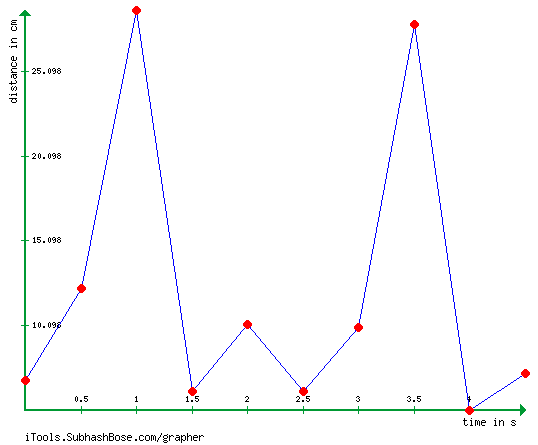
\includegraphics[scale=0.25]{Distance_Graph.png}
\caption{Ultrasonic Distance Graph}
\end{figure}
In Ultrasonic Sensor Alerting, we host an API i.e., host the sensor data acquisition code on a flask server. We make use of JavaScript to request sensor data from the API. Once the Ultrasonic Sensor readings are received, the data is then extracted and is in the JSON format. The data here being the distance.  We then make use of DOM manipulation to trigger alerts on the website application if the distance is less than 10cm.
The above figure represents the distance recorded in Real Time.

\section{Implementation of Robot Movement}
First the keystrokes are recorded using keyboard module in the form of a character,
the recorded characters are then sent from server to client using TCP/IP sockets.
Upon receiving the character on the receiver side the appropriate action is
implemented using an if-else ladder which is reflected by the motion of the robot.
Raspberry Pi GPIO used in Board mode and is connected to the motor driver in the format given below:
\begin{enumerate}[ ]
\item Pin 18 – IN1(Right)
\item Pin 16 – IN2(Right)
\item Pin 15 – IN3(Left)
\item Pin 13 – IN4(Left)
\item Pin 12 – ENA(PWM - Right)
\item Pin 33 – ENB(PWM - Left)
\end{enumerate}
\begin{figure}[h]
\centering
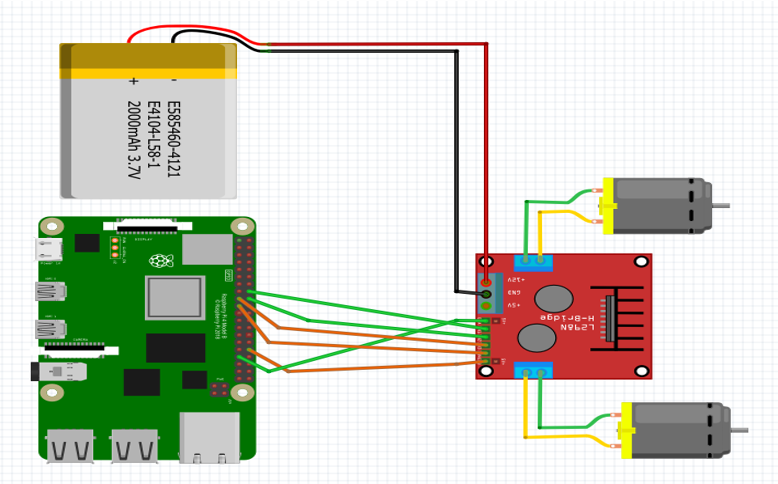
\includegraphics[scale=0.6]{ckt.png}
\caption{Motor Circuit Connections}
\end{figure}